\begin{figure*}[tb]
	\centering
	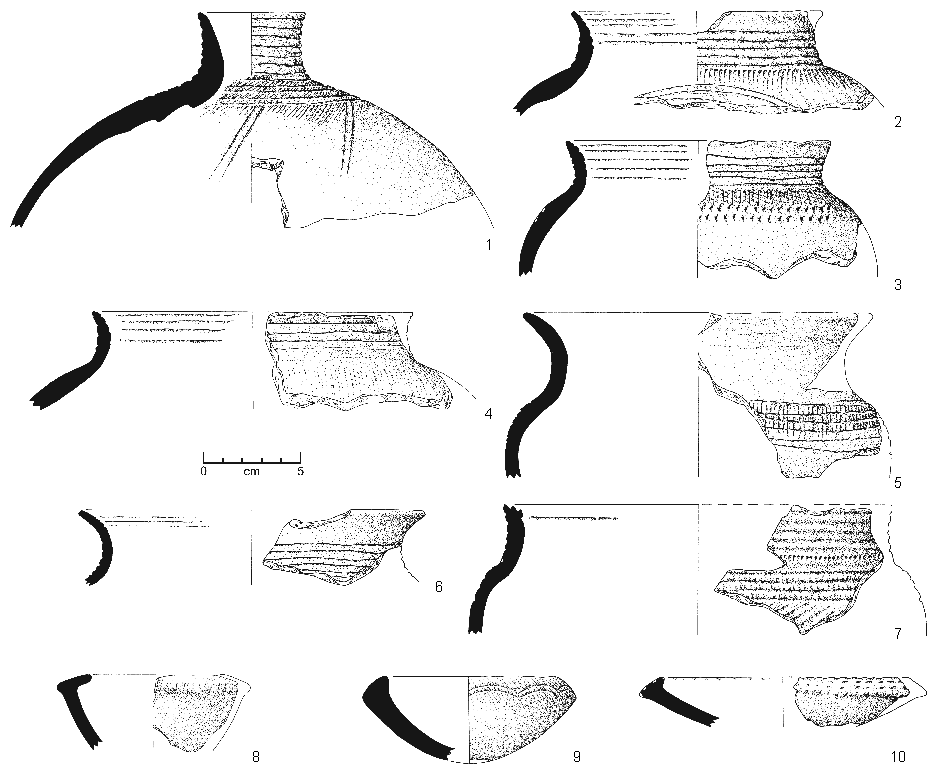
\includegraphics[width=.95\textwidth]{fig/KON-Typen.pdf}
	\caption{Konda-Gruppe: Typvertreter.\\1:~Taf.~61.1; 2~Taf.~61.2; 3:~Taf.~66.16; 4:~Taf.~61.4; 5:~Taf.~66.9; 6:~Taf.~66.19; 7:~Taf.~66.18.; 8:~Taf.~57.22; 9:~Taf.~60.24; 10:~Taf.~63.12.}
	\label{fig:KON_Typvertreter}
\end{figure*}

\subsubsection{Konda-Gruppe}\label{sec:KON-Gr}

Neben der Keramik der Mandombe-Gruppe (Kap.~\ref{sec:MDB-Gr}) sowie der noch zu beschreibenden Pandama-Keramik (Kap.~\ref{sec:PDM-Gr}) ließ sich eine weitere, vornehmlich am oberen \mbox{Sangha} sowie dem \mbox{Ngoko} verbreitete, keramische Stilgruppe herausarbeiten. Diese, nach dem Fundplatz Konda am oberen \mbox{Sangha} (Fpl.~268) benannte Gruppe, zeichnet sich durch Gefäße mit geschweiftem Profil und konkav ausbiegenden, häufig außen wie innen mit Rillen verzierten Rändern aus (Abb.~\ref{fig:KON_Typvertreter}). Überdies konnten eine große Anzahl kleiner, rundbodiger Schalen beobachtet werden, deren Verzierung sich in das Schema der größeren Gefäße einpasst und die in der Folge ebenfalls der Konda-Gruppe zugerechnet wurden.\footnote{Eine größere Anzahl vergleichbarer Schalen wurde in den späten 1990er Jahren bei Prospektionen im Südosten der Republik Kamerun, die als Fortsetzung des \textit{River Reconnaissance Project} unter der Leitung von Manfred~K.~H. Eggert durchgeführt wurden, entdeckt. Eine eingehende Auswertung dieser Feldarbeiten liegt bislang nicht vor. Grundsätzlich vergleichbare Formen finden sich auch im Fundmaterial des Inneren Kongobeckens. Während ein Stück aus Mbandaka \parencite[Fpl.~10, ][445 Taf. 11.3]{Wotzka.1995} der Bondongo- oder Mbandaka-Gruppe zugeordnet wird (ebd. 426), ist ein weiteres aus Nkile am Ruki (Fpl.~17; ebd. 465 Taf. 31.2--3 der Botendo-Gruppe zuzurechnen (ebd. 428).\label{ftn:KON-PDM_klSchalen}} 

Insgesamt können 156~GE aus 21 verschiedenen Fundplätzen der Kondo-Gruppe zugewiesen werden. Das Material stammt zu 97\,\% aus Absammlungen von Oberflächenkomplexen. Einzelne GE des Konda-Stils wurden in den drei in Pikunda am \mbox{Sangha} (Fpl.~255) ausgegrabenen Befunden (Kat.-Nr.~8--10) sowie in der Grube MUN~87/1 (Kat.-Nr.~15) in Munda am \mbox{Likwala}-\mbox{aux}-\mbox{Herbes} (Fpl.~304) erfasst. Die erste Beschreibung der Konda-Keramik erfolgte größtenteils an Randstücken. Sie machen mit 107~GE (70\,\%) auch das Gros dieser Stilgruppe aus. Ein nahezu vollständiges Gefäß, eine kleine Schale (Taf.~60.24) sowie 47 Fragmente von Gefäßwandungen (30\,\%) bilden den Rest der die Stilgruppe repräsentierenden GE. Bodenstücke sind nicht beobachtet worden. Das Material setzt sich größtenteils aus stark fragmentierten Stücken zusammen. Insgesamt 85\,\% aller Stücke sind kleiner als 70$\times$70\,mm und lediglich eine GE ist größer als 120$\times$120\,mm.


\paragraph{Technologische Merkmale}\hspace{-.5em}|\hspace{.5em}%
Die Scherben der Konda-Gruppe zeichnen sich durch einen deutlichen Anteil nichtplastischer Partikel aus. Über 90\,\% aller Stücke enthalten 25--40\,\% nichtplastische Partikel. Nur in geringem Umfang kommen auch Stücke mit unter 5\,\% Anteil nichtplastischer Partikel im Scherben vor. Die beobachteten Partikel sind fast ausschließlich den Größenklassen \textit{medium} (24\,\%), \textit{coarse} (54\,\%) sowie \textit{very coarse} (19\,\%) zuzurechnen. Es handelt sich vor allem um Quarzsand (77\,\%), der teilweise mit Laterit, Glimmer, Organik oder auch Schamott-Partikeln durchmischt ist. Das Gros ist den \textit{Fabrics} 3 (56\,\%) sowie 4 (27\,\%) zuzurechnen. Mit jeweils weniger als 6\,\% sind die \textit{Fabrics} 5, 7 und 8 vertreten. Mit Blick auf die Brennfarbe des genutzten Tones lassen sich, aufgrund beiger oder grauer Farbe, für 44\,\% der Stücke keine Angaben machen. Stücke, die auf die Nutzung rotbrennender Tone hindeuten, sind mit 26\,\% nur etwas seltener vertreten als solche, die weißbrennende Tone anzeigen. Diese machen 30\,\% aller GE der Konda-Gruppe aus. Die Oberflächen der Scherben sind sehr häufig leicht rau (55\,\%) oder rau (24\,\%).

\begin{figure*}[p]
	\centering
	\includegraphics[width=\textwidth]{fig/KON_Verbreitung.pdf}
	\caption{Konda-Gruppe: Verbreitung \parencite[grau nach][510 Abb.~3]{Eggert.2002}.}
	\label{fig:KON_Verbreitung}
\end{figure*}

\paragraph{Formen}\hspace{-.5em}|\hspace{.5em}%
Bei insgesamt 66~GE der Konda-Gruppe konnte die Gefäßform bestimmt werden, wobei für 21\,\% die Ansprache aufgrund schlechter Erhaltung nur unter Vorbehalt erfolgte. Gefäße mit stark konvexer Wandung, ohne ausgeprägten Halsbereich und konkav ausbiegendem Rand vom Typ D1 machen 33\,\% der beobachteten Formen aus (Abb.~\ref{fig:KON_Typvertreter}.2--7). Die Gefäße weisen maximale Bauchdurchmesser zwischen 12--27\,cm auf, jedoch konnte die Höhe der Mündung bei keiner GE hinreichend rekonstruiert werden. Neben der Gefäßform zeichnen sich diese GE durch einen konkaven, kurzen Gefäßhals aus, der direkt in einen konkav ausbiegenden Rand übergeht und innen wie außen mit horizontalen Rillen verziert ist. Diese Kombination aus Gefäßform, Randgestaltung und Verzierung ist maßgeblich für die Zuordnung von GE zur Konda-Gruppe. Die Konda-Gruppe zeichnet sich überdies durch das zahlreiche Auftreten zumeist kleiner, rundbodiger Schalen mit häufig T-förmig umgelegten Rändern aus (Abb.~\ref{fig:KON_Typvertreter}.8--10). Diese machen insgesamt 48\,\% aller der Konda-Gruppe zugerechneten GE aus. Sie weisen Durchmesser zwischen 12--27~cm auf und sind zwischen 1,5--11,5\,cm hoch. Die Ränder dieser Schalen sind entweder nur nach außen oder T-förmig, nach innen wie außen umgelegt. Ansprachen zum Gefäßboden ließen sich ausschließlich bei diesen Schalen machen und es wurden nur runde Böden beobachtet. In einem Fall konnte eine GE als Flasche identifiziert werden (Abb.~\ref{fig:KON_Typvertreter}.1). Dieses Stück entspricht, bis auf den stark verengten Gefäßhals, den Gefäßen mit konvexer Wandung vom Typ D1 der Konda-Gruppe.


\paragraph{Verzierungen}\hspace{-.5em}|\hspace{.5em}%
Bestimmendes Merkmal der Konda-Keramik ist der hohe Anteil an horizontalen Rillen (Tab.~\ref{tab:Verzierungselemente}: 02.1; 69\,\%), die sich fast ausschließlich innen wie außen am Rand sowie dem Gefäßhals befinden (Anlage~4\subref{fig:KON_Verz}). Daneben weist die Keramik -- deutlich seltener -- horizontale Reihen aus diagonalen (Tab.~\ref{tab:Verzierungselemente}: 04.12; 5\,\%), vertikal stehenden (Tab.~\ref{tab:Verzierungselemente}: 04.15; 5\,\%) oder runden Eindrücken (Tab.~\ref{tab:Verzierungselemente}: 04.11; 2\,\%) sowie diagonalen Kammstrich auf (Tab.~\ref{tab:Verzierungselemente}: 15.1; 4\,\%). Sechs GE sind zudem mit vegetabilischem \mbox{Roulette} verziert, in fünf Fällen handelt es sich um \textit{knotted string}- (Tab.~\ref{tab:Verzierungselemente}: 21.1; Abb.~\ref{fig:KON_Typvertreter}.7) und in einem Fall um \textit{twisted string}-\mbox{Roulette} (Tab.~\ref{tab:Verzierungselemente}: 21.2). Die Rouletteverzierung findet sich in allen Fällen auf dem Gefäßbauch oder der Schulter und tritt immer in Kombination mit anderen Verzierungselementen auf (Anlage~4\subref{fig:KON_Verz}). Trotz des Vorkommens von \mbox{Roulette} wird die Verzierung der Konda-Keramik vor allem von innen wie außen an Rand und Hals der Gefäße zu findenden Riefen und Rillen bestimmt.

\paragraph{Datierung}\hspace{-.5em}|\hspace{.5em}%
Für die Keramik der Konda-Gruppe liegen keine direkten Radiokohlenstoffdatierungen vor. Unter Vorbehalt der Konda-Gruppe zurechenbare GE wurden in allen drei Grabungsschnitten in Pikunda am mittleren \mbox{Sangha} (Fpl.~255) erfasst. Während das Inventar der rezenten Grube PIK~87/2 (Kat.-Nr.~9) eindeutig vermischt ist und die Fundzusammenhänge durch das Fehlen der Dokumentation des als PIK~87/3 (Kat.-Nr.~10) ausgegrabenen Metallurgiebefundes\footnote{Eine Datierung weist diesen Befund grob in das 11.--13.~Jh. n.~Chr. (KI-2892).} nicht mehr zweifelsfrei belegbar sind, liefern lediglich die Einzelfunde aus der jüngeren Grube A in PIK~87/1 (Kat.-Nr.~8) einen Datierungsansatz. Das vornehmlich durch die Keramik der Mandombe-Gruppe (Kap.~\ref{sec:MDB-Gr}) charakterisierte Inventar datiert in das 13.--15.~Jh. n.~Chr. (KI-2891). Diese Datierung deutet zumindest eine partielle Gleichzeitigkeit mit der Keramik der Mandombe-Gruppe an. Das Auftreten von Rouletteverzierung, die in größerem Umfang erst mit der mutmaßlich jüngeren Pandama-Gruppe (Kap.~\ref{sec:PDM-Gr}) aufkommt, deutet hingegen auf ein tendenziell jüngeres Alter im Vergleich zur Mandombe-Keramik. Die grundsätzliche Morphologie der Gefäße und vor allem  die rillenverzierten Gefäßhälse und Ränder deuten einen losen Bezug zur Keramik der Bobulu-Gruppe (Kap.~\ref{sec:BBL-Gr}) des \mbox{Ubangi}-Gebiets an.

\paragraph{Verbreitung}\hspace{-.5em}|\hspace{.5em}%
Die Verbreitung der Konda-Gruppe beschränkt sich auf einen eng begrenzten Bereich entlang des Oberlaufs des \mbox{Sangha} sowie des prospektierten Abschnitts des \mbox{Ngoko} (Abb.~\ref{fig:KON_Verbreitung}).\footnote{Ähnliche, bislang unveröffentlichte Stücke fanden sich auch bei der Wiederaufnahme der Feldarbeiten durch Manfred~K.~H.~Eggert im Südosten der Republik Kamerun in den späten 1990er Jahren \parencite[siehe][]{Eggert.2002} in Mokounounou (Obj. MKN~97/1:15 ) und Tala-Tala (Obj. TLT~97/101:71). Zur Zeit der Materialaufnahme für diese Arbeit war diese kamerunische Keramik in Tübingen eingelagert und nur eingeschränkt zugänglich.\label{ftn:SOKamerun1997Funde}} Keramik der Konda-Gruppe wurde an insgesamt 21 Fundplätzen beobachtet, wobei Ngama (Fpl.~281) den westlichsten, Leme (Fpl.~269) den nördlichsten und Molanda (Fpl.~258) den südlichsten Fundpunkt bildet.\footnote{Fragliche oder nur unter Vorbehalt der Konda-Gruppe zuweisbare Stücke fanden sich auch in Ngombe am \mbox{Sangha} (Fpl.~252; siehe Anm.~\ref{ftn:Vermischungen}) sowie Mosenge (Fpl.~299) und Munda (Fpl.~304) am oberen Likwala-aux-Herbes.}